\input{"preamble.tex"}

\addbibresource{NumberTheory.bib}

\let\Begin\begin
\let\End\end
\newcommand\wrapenv[1]{#1}

\makeatletter
\def\ScaleWidthIfNeeded{%
 \ifdim\Gin@nat@width>\linewidth
    \linewidth
  \else
    \Gin@nat@width
  \fi
}
\def\ScaleHeightIfNeeded{%
  \ifdim\Gin@nat@height>0.9\textheight
    0.9\textheight
  \else
    \Gin@nat@width
  \fi
}
\makeatother

\setkeys{Gin}{width=\ScaleWidthIfNeeded,height=\ScaleHeightIfNeeded,keepaspectratio}%

\title{
\rule{\linewidth}{1pt} \\
\textbf{
    Algebraic Number Theory
  }
    \\ {\normalsize Lectures by Paul Pollack. University of Georgia,
Spring 2021} \\
  \rule{\linewidth}{2pt}
}
\titlehead{
    \begin{center}
  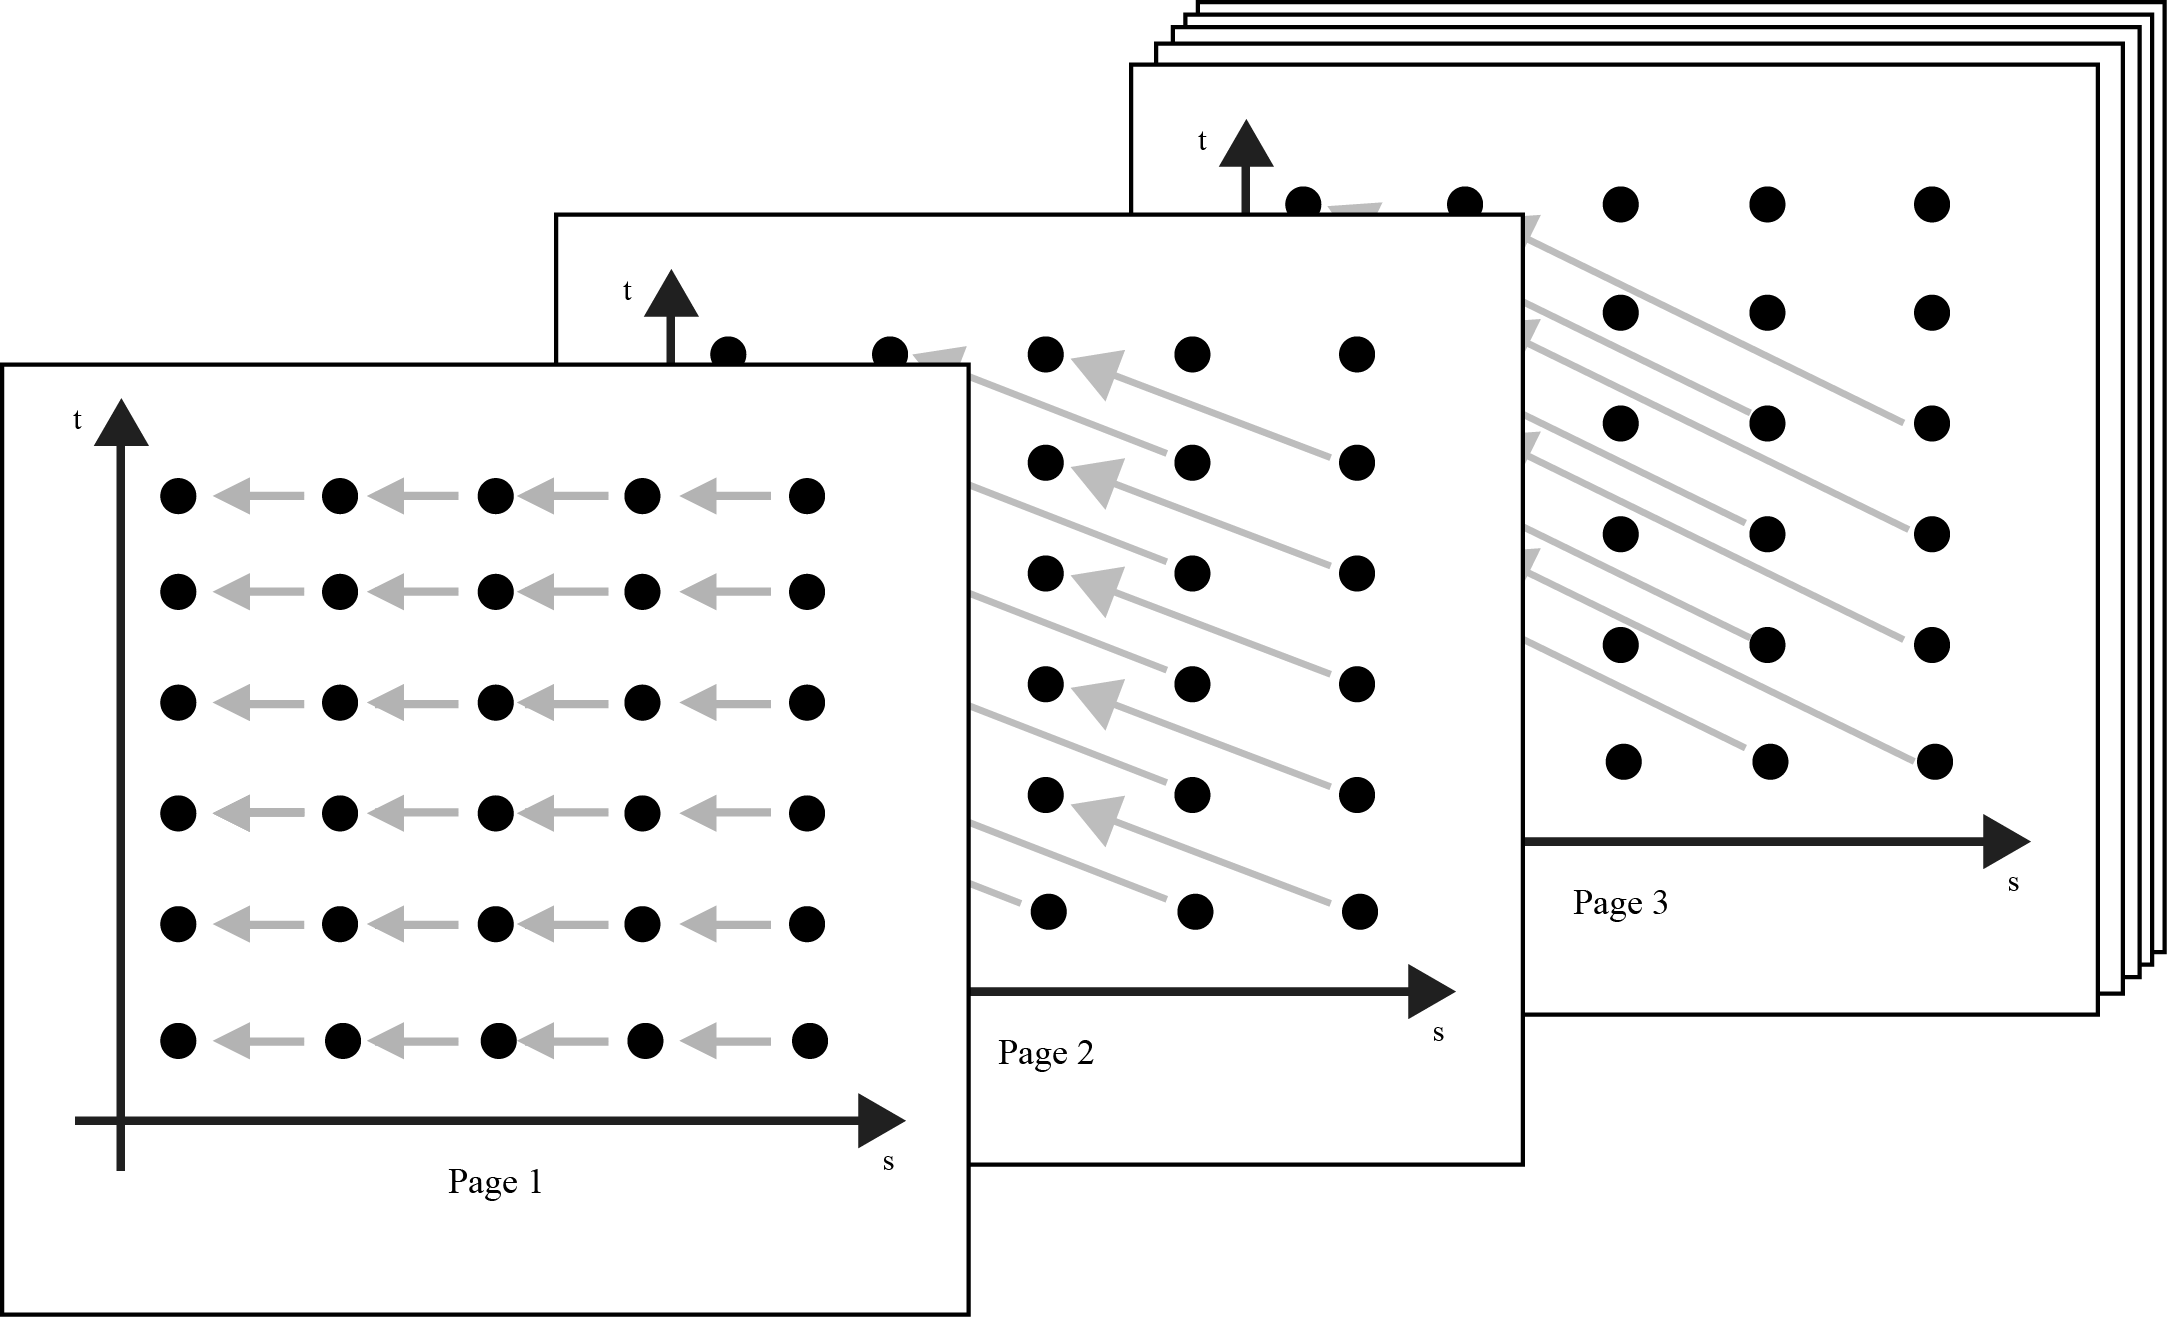
\includegraphics[width=\linewidth,height=0.45\textheight,keepaspectratio]{figures/cover.png}
  \end{center}
       \begin{minipage}{.35\linewidth}
    \begin{flushleft}
      \vspace{2em}
      {\fontsize{6pt}{2pt} \textit{Notes: These are notes live-tex'd
from a graduate course in Algebraic Number Theory taught by Paul Pollack
at the University of Georgia in Spring 2021. As such, any errors or
inaccuracies are almost certainly my own. } } \\
    \end{flushleft}
    \end{minipage}
    \hfill
    \begin{minipage}{.65\linewidth}
    \end{minipage}
  }







\begin{document}

\date{}
\author{D. Zack Garza}
\maketitle
\begin{flushleft}
\textit{D. Zack Garza} \\
\textit{University of Georgia} \\
  \textit{\href{mailto: dzackgarza@gmail.com}{dzackgarza@gmail.com}} \\
{\tiny \textit{Last updated:} 2021-01-26 }
\end{flushleft}


\newpage

% Note: addsec only in KomaScript
\addsec{Table of Contents}
\tableofcontents
\newpage

\def\contradiction
{
\tikz[baseline, x=0.2em, y=0.2em, line width=0.04em]
\draw (0,0) -- ({4*cos(45)},{4*sin(45)})
    (-1,1) -- ({-1 + 4*cos(45)},{1 + 4*sin(45)})
    (-1,3) -- ({-1 + 4*cos(315)},{3 + 4*sin(315)})
    (0,4) -- ({0 + 4*cos(315)},{4 + 4*sin(315)});
}

\hypertarget{thursday-january-14}{%
\section{Thursday, January 14}\label{thursday-january-14}}

See website for notes on books, intro to class.

\begin{itemize}
\item
  Youtube Playlist:
  \url{https://www.youtube.com/playlist?list=PLA0xtXqOUji8fjQysx4k8a6h-hOZ7x5ue}
\item
  Free copies of textbook:
  \url{https://www.dropbox.com/sh/rv5j222kn74bjhm/AABZ1qcR1rOnpaBsa5CL3P_Ea?dl=0\&lst=}
\item
  Course website: ?
\end{itemize}

Paul's description of the course:

``This course is an introduction to arithmetic''beyond
\({\mathbb{Z}}\)``, specifically arithmetic in the ring of''integers" in
a finite extension of \({\mathbb{Q}}\). (Among many other things) we'll
prove three important theorems about these rings:

\begin{itemize}
\tightlist
\item
  Unique factorization into ideals.
\item
  Finiteness of the group of ideal classes.
\item
  Dirichlet's theorem on the structure of the unit group."
\end{itemize}

\hypertarget{motivation}{%
\subsection{Motivation}\label{motivation}}

Solving Diophantine equations, i.e.~polynomial equations over
\({\mathbb{Z}}\).

\begin{example}[?]

Consider \(y^2 = x^3 + x\).

\begin{claim}

\((x, y) = (0, 0)\) is the only solution.

\end{claim}

To see this, write \(y^2 = x(x^2+1)\), which are relatively prime,
i.e.~no \(D\in {\mathbb{Z}}\) divides both of them. Why? If
\(d \divides x\) and \(d \divides x+1\), then
\(d\divides (x^2+1) + (-x) = 1\). It's also the case that both \(x^2+1\)
and \(x^2\) are squares (up to a unit), so \(x^2, x^2 + 1\) are
consecutive squares in \({\mathbb{Z}}\). But the gaps between squares
are increasing: \(1, 2, 4, 9, \cdots\). The only possibilities would be
\(x=0, y=1\), but in this case you can conclude \(y=0\).

\end{example}

\begin{example}[Fermat]

Consider \(y^2 = x^3-2\).

\begin{claim}

\((3, \pm 5)\) are the only solutions.

\end{claim}

Rewrite
\begin{align*}
x^3 = y^2+2 &= (y+ \sqrt{-2})(y - \sqrt{-2}) \\ 
&\in
{\mathbb{Z}}[\sqrt{-2}] \coloneqq\left\{{a+b\sqrt{-2} {~\mathrel{\Big|}~}a,b,\in {\mathbb{Z}}}\right\} \leq {\mathbb{C}}
.\end{align*}
This is a subring of \({\mathbb{C}}\), and thus at least an integral
domain. We want to try the same argument: showing the two factors are
relatively prime. A little theory will help here:

\begin{definition}[Norm Map]

For \(\alpha\in {\mathbb{Z}}[\sqrt{-2}]\) define
\(N \alpha = \alpha\mkern 1.5mu\overline{\mkern-1.5mu\alpha\mkern-1.5mu}\mkern 1.5mu\).

\end{definition}

\begin{lemma}[?]

Let \(\alpha, \beta \in {\mathbb{Z}}[\sqrt{-2}]\). Then

\begin{enumerate}
\def\labelenumi{\arabic{enumi}.}
\item
  \(N(\alpha \beta) = N(\alpha) N(\beta)\)
\item
  \(N( \alpha) \in {\mathbb{Z}}_{\geq 0}\) and \(N(\alpha) = 0\) if and
  only if \(\alpha= 0\).
\item
  \(N(\alpha) = 1 \iff \alpha\in R^{\times}\)
\end{enumerate}

\end{lemma}

\begin{proof}[?]

\begin{enumerate}
\def\labelenumi{\arabic{enumi}.}
\item
  Missing, see video (10:13 AM).
\item
  \(N(\alpha) = a^2 + 2b^2 \geq 0\), so this equals zero if and only if
  \(\alpha= \beta= 0\)
\item
  Write
  \(1 = \alpha\mkern 1.5mu\overline{\mkern-1.5mu\alpha\mkern-1.5mu}\mkern 1.5mu\)
  if \(N(\alpha) = 1 \in R^{\times}\). Conversely if
  \(\alpha\in R^{\times}\) write \(\alpha \beta = 1\), then
  \begin{align*} 
  1 = N(1) = N(\alpha \beta) = N(\alpha ) N(\beta ) \in {\mathbb{Z}}_{\geq 0} 
  ,\end{align*}
  which forces both to be 1.
\end{enumerate}

\end{proof}

\begin{claim}

The two factors \(y \pm \sqrt 2\) are \emph{coprime} in
\({\mathbb{Z}}[\sqrt{-2}]\), i.e.~every common divisor is a unit.

\end{claim}

\begin{proof}[?]

Suppose \(\delta\divides y\pm \sqrt{-2}\), then
\(y + \sqrt{-2} = \delta \beta\) for some
\(\beta\in {\mathbb{Z}}[\sqrt{-2}]\). Take norms to obtain
\(y^2 + 2 = N \delta N \beta\), and in particular

\begin{itemize}
\tightlist
\item
  \(N \delta y^2 +2\)
\item
  \(\delta \divides (y+ \sqrt{-2} ) - (y - \sqrt{-2} ) = 2 \sqrt{-2}\)
  and thus \(N \delta \divides N(2 \sqrt{-2} ) = 8\).
\end{itemize}

In the original equation \(y^2 = x^3-2\), if \(y\) is even then \(x\) is
even, and \(x^3 - 2 \equiv 0-2 \pmod 4 \equiv 2\), and so
\(y^2 \equiv 2 \pmod 4\). But this can't happen, so \(y\) is odd, and
we're done: we have \(N \delta\divides 8\) which is even or 1, but
\(N \delta\divides y^2 +2\) which is odd, so \(N \delta = 1\).

\end{proof}

We can identify the units in this ring:
\begin{align*}
{\mathbb{Z}}[\sqrt{-2} ]^{\times}= \left\{{ a + b \sqrt{-2} {~\mathrel{\Big|}~}a^2 + 2b^2 = 1}\right\}
\end{align*}
which forces \(a^2 \leq 1, b^2 \leq 1\) and thus this set is
\(\left\{{\pm 1}\right\}\).

So we have \(x^3 = ab\) which are relatively primes, so \(a,b\) should
also be cubes. We don't have to worry about units here, since \(\pm 1\)
are both cubes. So e.g.~we can write
\begin{align*}
y + \sqrt{-2} = (a + b \sqrt{-2} )^3 = (a^3-6ab^2) + (3a^2b -2b^3) \sqrt{-2}
.\end{align*}
Comparing coefficients of \(\sqrt{-2}\) yields
\begin{align*} 1 = b(3a^2b - 2b^2) \in {\mathbb{Z}}\implies b \divides 1
,\end{align*}
and thus \(b\in {\mathbb{Z}}^{\times}\),
i.e.~\(b\in \left\{{\pm 1}\right\}\). By cases:

\begin{itemize}
\item
  If \(b=1\), then \(1 = 3a^2 -2 \implies a^2 = 1 \implies a = \pm 1\).
  So
  \begin{align*}
  y = \sqrt{-2} = (\pm 1 + \sqrt{-2} )^3 = \pm 5 + \sqrt{-2}
  ,\end{align*}
  which forces \(y=\pm 5\), the solution we already knew.
\item
  If \(b = -1\), then \(1 = -(3a^2 - 1)\) which forces
  \(1=3a^2 \in {\mathbb{Z}}\), so there are no solutions.
\end{itemize}

\end{example}

\begin{example}[?]

Consider \(y^2 = x^3 - 26\). Rewrite this as
\begin{align*}
x^3 = y^2 + 26 = (y + \sqrt{-26} )(y - \sqrt{-26} )
,\end{align*}
then the same lemma goes through with \(2\) replaced by \(26\)
everywhere where the RHS factors are still coprime. Setting
\(y + \sqrt{-26} = (a + b \sqrt{-26} )^3\) and comparing coefficients,
you'll find \(b=1, a = \pm 3\). This yields \(x=35, y=\pm 207\). But
there are more solutions: \((x, y) = (3, \pm 1)\)! The issue is that we
used unique factorization when showing that \(ab\) is a square implies
\(a\) or \(b\) is a square (say by checking prime factorizations and
seeing even exponents). In this ring, we can have \(ab\) a cube with
\emph{neither} \(a,b\) a cube, even up to a unit.

\end{example}

\begin{question}

When does a ring admit unique factorization? Do you even \emph{need} it?

\end{question}

This will lead to a discussion of things like the \textbf{class number},
which measure the failure of unique factorization. In general, the above
type of proof will work when the class number is 3!

\hypertarget{lecture-2-tuesday-january-19}{%
\section{Lecture 2 (Tuesday, January
19)}\label{lecture-2-tuesday-january-19}}

Today: Ch.2 of the book, ``Cast of Characters''. Note that all rings
will be commutative and unital in this course.

Last time: looked at factorization in
\({\mathbb{Z}}[\sqrt 2], {\mathbb{Z}}[\sqrt{26}]\). Where do rings like
this come from?

\begin{definition}[Number Field]

A \textbf{number field} is a subfield \(K \subseteq {\mathbb{C}}\) such
that \([K: {\mathbb{Q}}] < \infty\).

\end{definition}

\begin{remark}

Some authors don't require \(K \subseteq {\mathbb{C}}\), but any finite
extension of \({\mathbb{Q}}\) will embed into \({\mathbb{C}}\) so
there's no harm in this extra requirement.

\end{remark}

\begin{example}[?]

\({\mathbb{Q}}[\sqrt[3]{2}, {\mathbb{Q}}[\sqrt 2, \sqrt[5]{7}]\) or
\({\mathbb{Q}}(\theta)\) where \(\theta\) is a root of \(x^5 - x - 1\)
(which you can check is irreducible. Now that the round vs.~square
brackets here won't make a difference, since we're adjoining algebraic
numbers.

\end{example}

\begin{proposition}[?]

Let \(K_{/{\mathbb{Q}}}\) be a finite extension, say of degree
\(n\coloneqq[K: {\mathbb{Q}}]\). Then there are \(n\) distinct
embeddings \footnote{An injective ring morphism.} of \(K\) into
\({\mathbb{C}}\)

\end{proposition}

\begin{proof}[?]

We have \(K_{/{\mathbb{Q}}}\), which is necessarily separable since
\(\operatorname{ch}({\mathbb{Q}}) = 0\). By the primitive element
theorem, we can write \(K = {\mathbb{Q}}(\theta)\) where \(\theta\) is a
root of some degree \(n\) irreducible polynomial
\(f(x) \in {\mathbb{Q}}[x]\). Since \({\mathbb{C}}\) is algebraically
closed, \(f\) splits completely over \({\mathbb{C}}\) as
\(f = \prod_{i=1}^n (x- \theta_i\) which each \(\theta_i \in CC\)
distinct since \(f\) was irreducible and we're in characteristic zero.
Then for each \(i\) there is an embedding \(K = {\mathbb{Q}}[\theta]\)
given by
\begin{align*}
\iota_i: {\mathbb{Q}}[\theta] &\hookrightarrow{\mathbb{C}}\\
g(\theta) &\mapsto g(\theta_i)
.\end{align*}
There are some easy things to check:

\begin{itemize}
\tightlist
\item
  This is well-defined: elements in \(K\) are polynomials in \(\theta\)
  but they all differ by a multiple of the minimal polynomial of
  \(\theta\),
\item
  This is an inject homomorphism and thus an embedding, and
\item
  For distinct \(i\) you get distinct embeddings: just look at the image
  \(\iota_i(\theta)\), these are distinct numbers in \({\mathbb{C}}\).
\end{itemize}

\end{proof}

\begin{definition}[Real and Nonreal embeddings]

Let \(K_{/{\mathbb{Q}}}\) be a finite extension of degree
\(n = [K : {\mathbb{Q}}]\). We'll say an embedding
\(\sigma:K \to {\mathbb{C}}\) is \textbf{real} if
\(\sigma(K) \subseteq {\mathbb{R}}\) , otherwise we'll say the embedding
is \textbf{nonreal}.

\end{definition}

\begin{remark}

If \(\sigma\) is a nonreal, then
\(\mkern 1.5mu\overline{\mkern-1.5mu\sigma\mkern-1.5mu}\mkern 1.5mu\) is
a nonreal embedding, so this embeddings come in pairs. As a consequence,
the total number of embeddings is given by \(n = r_1 + 2r_2\), where
\(r_1\) is the number of real embeddings and \(r_2\) is the number of
nonreal embeddings.

\end{remark}

\begin{example}[?]

Let \(K = {\mathbb{Q}}(\sqrt[3]{2})\). Here \(n=3\) since this is the
root of a degree 3 irreducible polynomial. Using the proof we can find
the embeddings: factor
\begin{align*}
x^3 - 2 = (x - \sqrt[3]{2})(x - \omega \sqrt[3]{2}) (x - \omega^2 \sqrt[3]{2})
.\end{align*}
where \(\omega = e^{2\pi i / 3}\) is a complex cube root of unity. We
can form an embedding by sending
\(\sqrt[3]{2} \to \omega^j \sqrt[3]{2}\) for \(j=0,1,2\). The case
\(j=0\) sends \(K\) to a subset of \({\mathbb{R}}\) and yields a real
embedding, but the other two will be nonreal. So \(r_1 = 1, r_2 = 1\),
and we have \(3 = 1 + 2(1)\) and this is consistent.

\end{example}

\begin{remark}

We've only been talking about fields, since unique factorization is
trivial since there are no primes. There are thus ``too many'' units,
compared to the rings we were considering before, so we'll restrict to
subrings. The question is: where is the arithmetic? Given a number field
\(K\), we want a ring \({\mathbb{Z}}_K\) that fits this analogy:

\begin{center}
\begin{tikzcd}
{\mathbb{Q}}\ar[dd] & \leadsto & K\ar[dd] \\
\\
{\mathbb{Z}}& \leadsto & {\mathbb{Z}}_K = ?
\end{tikzcd}
\end{center}

\end{remark}

\begin{definition}[Algebraic Numbers]

Given \(\alpha\in {\mathbb{C}}\) we say \(\alpha\) is an
\textbf{algebraic number} if and only if \(\alpha\) is algebraic over
\({\mathbb{Q}}\), i.e.~the root of some polynomial in
\({\mathbb{Q}}[x]\).

\end{definition}

\begin{remark}

We know that if we define
\(\mkern 1.5mu\overline{\mkern-1.5mu{\mathbb{Q}}\mkern-1.5mu}\mkern 1.5mu\coloneqq\left\{{\alpha\in {\mathbb{C}}{~\mathrel{\Big|}~}\alpha \text{ is algebraic over } {\mathbb{Q}}}\right\}\),
we can alternatively describe this as
\(\mkern 1.5mu\overline{\mkern-1.5mu{\mathbb{Q}}\mkern-1.5mu}\mkern 1.5mu= \left\{{ \alpha\in {\mathbb{C}}{~\mathrel{\Big|}~}[{\mathbb{Q}}(\alpha) : {\mathbb{Q}}] < \infty }\right\}\).
This is convenient because it's easy to see that algebraic numbers are
closed under sums and products, just using the ways degrees behave in
towers.

\end{remark}

\begin{corollary}[?]

\(\mkern 1.5mu\overline{\mkern-1.5mu{\mathbb{Q}}\mkern-1.5mu}\mkern 1.5mu\hookrightarrow{\mathbb{C}}\)
is a subfield and every number field is a subfield of
\(\mkern 1.5mu\overline{\mkern-1.5mu{\mathbb{Q}}\mkern-1.5mu}\mkern 1.5mu\).

\end{corollary}

These are still fields, so lets define some interesting subrings.

\begin{definition}[$\bar \ZZ$ ]

Define
\(\mkern 1.5mu\overline{\mkern-1.5mu{\mathbb{Z}}\mkern-1.5mu}\mkern 1.5mu\coloneqq\left\{{ \alpha\in {\mathbb{C}}{~\mathrel{\Big|}~}\alpha\text{ is the root of a monic polynomial }f\in {\mathbb{Z}}[x]}\right\}\).

\end{definition}

\begin{theorem}[$\bar \ZZ$ is a ring]

\(\mkern 1.5mu\overline{\mkern-1.5mu{\mathbb{Z}}\mkern-1.5mu}\mkern 1.5mu\)
is a ring, and in fact a domain since it's a subring of
\({\mathbb{C}}\).

\end{theorem}

We'll use an intermediate criterion to prove this:

\begin{proposition}[Integrality Criterion]

Let \(\alpha\in {\mathbb{C}}\) and suppose there is a finitely generated
\({\mathbb{Z}}{\hbox{-}}\)submodule of \({\mathbb{C}}\) with
\(\alpha M \subseteq M \neq 0\). Then
\(\alpha\in \mkern 1.5mu\overline{\mkern-1.5mu{\mathbb{Z}}\mkern-1.5mu}\mkern 1.5mu\),
i.e.~\(\alpha\) is the root of a monic polynomial with integer
coefficients.

\end{proposition}

\begin{proof}[of integrality criterion]

Chasing definitions, take \(M\) and choose a finite list of generators
\(\beta_1, \beta_2, \cdots, \beta_m\) for \(M\). Then
\(\alpha M \subseteq M \implies \alpha \beta_i \in M\) for all \(M\),
and each \(\alpha \beta_i\) is a \({\mathbb{Z}}{\hbox{-}}\)linear
combination of the \(\beta_i\) . I.e. we have
\begin{align*}
\alpha 
\begin{bmatrix}
\beta_1 
\\
\vdots  
\\
\beta_n  
\end{bmatrix}
= 
\begin{bmatrix}
a_{11} & a_{12} & \cdots
\\
a_{21} &  a_{22} & 
\\
 \vdots &  &\ddots  
\end{bmatrix}
\begin{bmatrix}
\beta_1 
\\
\vdots  
\\
\beta_n  
\end{bmatrix}
\coloneqq A \vec{\beta}
,\end{align*}
where \(A \in \operatorname{Mat}(n\times m, {\mathbb{Z}})\). We can
rearrange this to say that
\begin{align*}
\qty{ \alpha \operatorname{id}- A} 
\begin{bmatrix}
\beta_1 
\\
\vdots  
\\
\beta_n  
\end{bmatrix}
=
\mathbf{0}
.\end{align*}
Not all of the \(\beta_i\) can be zero since \(M\neq 0\), and thus
\(\alpha \operatorname{id}- A\) is singular and thus has determinant
zero, so \(\det(x \operatorname{id}- A)\Big|_{x=a} = 0\). We have
\begin{align*}
x\operatorname{id}- A = 
\begin{bmatrix}
x - a_{1,} &  & &
\\
&  x - a_{2, 2} & & 
\\
&  & \ddots &
\\
& &  & x - a_{m, m}
\end{bmatrix}
,\end{align*}
where the off-diagonal components are constants in \({\mathbb{Z}}\)
coming from \(A\). Taking the determinant yields a monic polynomial: the
term of leading degree comes from multiplying the diagonal components,
and expanding over the remaining minors only yields terms of smaller
degree. So \(\det (x\operatorname{id}- A) \in {\mathbb{Z}}[x]\) is
monic.

\end{proof}

\begin{proof}[of theorem]

We want to show that
\(\mkern 1.5mu\overline{\mkern-1.5mu{\mathbb{Z}}\mkern-1.5mu}\mkern 1.5mu\)
is a ring, and it's enough to show that

\begin{itemize}
\tightlist
\item
  \(1\in \mkern 1.5mu\overline{\mkern-1.5mu{\mathbb{Z}}\mkern-1.5mu}\mkern 1.5mu\),
  which is true since \(x-1\) is monic.
\item
  It's closed under \(+, \cdot\).
\end{itemize}

Note that the first property generalizes to
\({\mathbb{Z}}\subseteq \mkern 1.5mu\overline{\mkern-1.5mu{\mathbb{Z}}\mkern-1.5mu}\mkern 1.5mu\),
since \(x-n\) is monic for any \(n\in {\mathbb{Z}}\). For the second,
let
\(\alpha, \beta \in \mkern 1.5mu\overline{\mkern-1.5mu{\mathbb{Z}}\mkern-1.5mu}\mkern 1.5mu\).
Define \(M \coloneqq{\mathbb{Z}}[\alpha, \beta]\), then it's clear that
\((\alpha + \beta)M \subseteq M\) and \((\alpha \beta)M \subseteq M\)
since \({\mathbb{Z}}[\alpha, \beta]\) are polynomials in
\(\alpha, \beta\) and multiplying by these expression still yields such
polynomials. It only remains to check the following:

\begin{claim}

\(M\) is finitely-generated.

\end{claim}

\begin{proof}[?]

Let \(\alpha\) be a root of \(f \in {\mathbb{Z}}[x]\) and \(\beta\) a
root of \(g\), both monic with \(\deg f = n, \deg g = m\). We want to
produce a finite generating set for
\(M\coloneqq{\mathbb{Z}}[\alpha, \beta]\), and the claim is that the
following works:
\(\left\{{ \alpha^i \beta^j}\right\} _{\substack{0\leq i < n \\ 0 \leq j < m} }\),
i.e.~every element of \(M\) is some \({\mathbb{Z}}{\hbox{-}}\)linear
combination of these.

Note that this is clearly true if we were to include \(n, m\) in the
indices by collecting terms of any polynomial in \(\alpha, \beta\), so
the restrictions are nontrivial. It's enough to show that for any
\(0 \leq I, J \in {\mathbb{Z}}\), the term \(\alpha^I \beta^J\) is a
\({\mathbb{Z}}{\hbox{-}}\)linear combination of the restricted elements
above. Divide by \(f\) and \(g\) to obtain \(x^I = f(x) q(x) + r(x)\)
and \(x^J = g(x) \tilde q(x) \tilde r(x)\) where \(r(x) = 0\) or
\(\deg r < n\) and similarly for \(\tilde r\), where (importantly) all
of these polynomials are in \({\mathbb{Z}}[x]\).

We're not over a field: \({\mathbb{Z}}[x]\) doesn't necessarily have a
division algorithm, so why is this okay? The division algorithm only
requires inverting the leading coefficient, so in general \(R[x]\)
admits the usual division algorithm whenever the leading coefficient is
in \(R^{\times}\).

Now plug \(\alpha\) into the first equation to obtain
\(\alpha^I = r(\alpha)\) where \(\deg r < n\), which rewrite
\(\alpha^I\) as a sum of lower-degree terms. Similarly writing
\(\beta^J = r(\beta)\), we can express
\begin{align*}
\alpha^I \beta^J = r(\alpha) r(\beta)
,\end{align*}
which is what we wanted.

\end{proof}

\end{proof}

\begin{remark}

We've just filled in another part of the previous picture:

\begin{center}
\begin{tikzcd}
{\mathbb{Q}}\ar[dd] & K\ar[dd] & \mkern 1.5mu\overline{\mkern-1.5mu{\mathbb{Q}}\mkern-1.5mu}\mkern 1.5mu\ar[dd]\\
\\
{\mathbb{Z}}& {\mathbb{Z}}_K & \mkern 1.5mu\overline{\mkern-1.5mu{\mathbb{Z}}\mkern-1.5mu}\mkern 1.5mu
\end{tikzcd}
\end{center}

\end{remark}

\begin{definition}[Ring of Integers]

Define
\({\mathbb{Z}}_K = \mkern 1.5mu\overline{\mkern-1.5mu{\mathbb{Z}}\mkern-1.5mu}\mkern 1.5mu\cap K\),
the \textbf{ring of integers} of \(K\). Note that this makes sense since
the intersection of rings is again a ring.

\end{definition}

\begin{remark}

Why not just work in
\(\mkern 1.5mu\overline{\mkern-1.5mu{\mathbb{Z}}\mkern-1.5mu}\mkern 1.5mu\)?
It doesn't have the factorization properties we want, e.g.~there are no
irreducible elements. Consider \(\sqrt 2\), we can factor is into two
non-units (noting that \(\sqrt 2\) is not a unit) as
\(\sqrt{\sqrt 2} \cdot \sqrt{\sqrt 2}\), and it's easy to check that if
\(a\) is not a unit then \(\sqrt a\) is not a unit. So this would yield
arbitrarily long factorizations, and is thus not Noetherian.

\end{remark}

The following is a reality check, and certainly a property we would
want:

\begin{proposition}[The ring of integers of $\QQ$ is $\ZZ$ ]

\({\mathbb{Z}}_{\mathbb{Q}}= {\mathbb{Z}}\).

\end{proposition}

\begin{proof}[of proposition]

\(\subseteq\): easy, since
\({\mathbb{Z}}\subseteq \mkern 1.5mu\overline{\mkern-1.5mu{\mathbb{Z}}\mkern-1.5mu}\mkern 1.5mu\)
and \({\mathbb{Z}}\subseteq {\mathbb{Q}}\), and is thus in their
intersection \({\mathbb{Z}}_{\mathbb{Q}}\) .

\(\supseteq\) : Let
\(\alpha\in {\mathbb{Z}}_{\mathbb{Q}}= {\mathbb{Q}}\cap\mkern 1.5mu\overline{\mkern-1.5mu{\mathbb{Z}}\mkern-1.5mu}\mkern 1.5mu\)
, so \(\alpha\) is a root of
\(x^n - a_{n-1}x^{n-1} + \cdots + a_1x + a_0 \in {\mathbb{Z}}[x]\). We
know \(\alpha= a/b\) with \(a,b \in {\mathbb{Z}}\), and we can use the
rational root test which tells us that \(a\divides a_0, b\divides 1\),
so \(b = \pm 1, \alpha = a/\pm 1 = \pm a \in {\mathbb{Z}}\) and thus
\(\alpha \in {\mathbb{Z}}\).

\end{proof}

We'll want to study \({\mathbb{Z}}_K\) for various number fields \(K\),
but we'll need more groundwork.

\begin{proposition}[Easy criterion to check if an integer is algebraic]

Let
\(\alpha \in \mkern 1.5mu\overline{\mkern-1.5mu{\mathbb{Q}}\mkern-1.5mu}\mkern 1.5mu\),
then
\begin{align*} \alpha\in \mkern 1.5mu\overline{\mkern-1.5mu{\mathbb{Z}}\mkern-1.5mu}\mkern 1.5mu\iff \min_ \alpha \in {\mathbb{Z}}[x], \end{align*}
where \(\min_ \alpha(x)\) is the unique monic irreducible polynomial in
\({\mathbb{Q}}[x]\) which vanishes at \(\alpha\).

\end{proposition}

\begin{proof}[?]

\(\impliedby\): Trivial, if the minimal polynomial already has integer
coefficients, just note that it's already monic and thus
\(\alpha \in \mkern 1.5mu\overline{\mkern-1.5mu{\mathbb{Z}}\mkern-1.5mu}\mkern 1.5mu\)
by definition.

\(\implies\): Why should the minimal polynomial have \emph{integer}
coefficients? Choose a monic \(f(x) \in {\mathbb{Z}}[x]\) with
\(f(\alpha) = 0\), using the fact that
\(\alpha\in \mkern 1.5mu\overline{\mkern-1.5mu{\mathbb{Z}}\mkern-1.5mu}\mkern 1.5mu\)
, and factor \(f(x) = \prod_{i=1}^n (x- \alpha_i) \in {\mathbb{C}}[x]\).
Note that each
\(\alpha_i \in \mkern 1.5mu\overline{\mkern-1.5mu{\mathbb{Z}}\mkern-1.5mu}\mkern 1.5mu\)
since they are all roots of \(f\) (a monic polynomial in
\({\mathbb{Z}}[x]\)). Use the fact that \(\min_ \alpha(x)\) divides
every polynomial which vanishes on \(\alpha\) over \({\mathbb{Q}}\), and
thus divides \(f\) (noting that this still divides over
\({\mathbb{C}}\)). Moreover, every root of \(\min_ \alpha(x)\) is a root
of \(f\), and so every such root is some \(\alpha_i\).

Now factor \(\min_ \alpha(x)\) over \({\mathbb{C}}\) to obtain
\(\min_ \alpha(x) = \prod_{i=1}^m (x - \beta_i)\) with all of the
\(\beta_i \in \mkern 1.5mu\overline{\mkern-1.5mu{\mathbb{Z}}\mkern-1.5mu}\mkern 1.5mu\).
What coefficients appear after multiplying things out? Just sums and
products of the \(\beta_i\), so all of the coefficients are in
\(\mkern 1.5mu\overline{\mkern-1.5mu{\mathbb{Z}}\mkern-1.5mu}\mkern 1.5mu\)
. Thus
\(\min_ \alpha(x) \in \mkern 1.5mu\overline{\mkern-1.5mu{\mathbb{Z}}\mkern-1.5mu}\mkern 1.5mu[x]\).
But the coefficients are also in \({\mathbb{Q}}\) by definition, so the
coefficients are in
\(\mkern 1.5mu\overline{\mkern-1.5mu{\mathbb{Z}}\mkern-1.5mu}\mkern 1.5mu\cap{\mathbb{Q}}= {\mathbb{Z}}\)
and thus \(\min_ \alpha(x) \in {\mathbb{Z}}[x]\).

\end{proof}

\begin{example}[Showing an integer is not algebraic using minimal polynomials]

\(\sqrt{5}/ 3 \not\in \mkern 1.5mu\overline{\mkern-1.5mu{\mathbb{Z}}\mkern-1.5mu}\mkern 1.5mu\)
since \(\min_ \alpha(x) = x^2 - 5/9 \not\in {\mathbb{Z}}[x]\), so this
is not an algebraic integer.

\end{example}

\begin{proposition}[$\ff(\ZZ_K) = K$ ]

\envlist

\begin{enumerate}
\def\labelenumi{\alph{enumi}.}
\tightlist
\item
  \(\mkern 1.5mu\overline{\mkern-1.5mu{\mathbb{Z}}\mkern-1.5mu}\mkern 1.5mu\)
  has
  \(\mkern 1.5mu\overline{\mkern-1.5mu{\mathbb{Q}}\mkern-1.5mu}\mkern 1.5mu\)
  as its fraction field, and
\item
  For any number field \(K\), \({\mathbb{Z}}_K\) has \(K\) as its
  fraction field.
\end{enumerate}

Moreover, both of these statements follow from:

\begin{enumerate}
\def\labelenumi{\alph{enumi}.}
\setcounter{enumi}{2}
\tightlist
\item
  If
  \(\alpha\in \mkern 1.5mu\overline{\mkern-1.5mu{\mathbb{Q}}\mkern-1.5mu}\mkern 1.5mu\)
  then
  \(d \alpha\in \mkern 1.5mu\overline{\mkern-1.5mu{\mathbb{Z}}\mkern-1.5mu}\mkern 1.5mu\)
  for some \(d\in {\mathbb{Z}}^{\geq 0}\)
\end{enumerate}

\end{proposition}

\begin{remark}

Thus the subring is ``big'' in the sense that if you allow taking
quotients, you recover the entire field. That \(c\implies a,b\): suppose
you want to write
\(\alpha \in \mkern 1.5mu\overline{\mkern-1.5mu{\mathbb{Q}}\mkern-1.5mu}\mkern 1.5mu\)
as \(\alpha=p/q\) with
\(p,q \in \mkern 1.5mu\overline{\mkern-1.5mu{\mathbb{Z}}\mkern-1.5mu}\mkern 1.5mu\).
Use \(c\) to produce
\(d\alpha\in \mkern 1.5mu\overline{\mkern-1.5mu{\mathbb{Z}}\mkern-1.5mu}\mkern 1.5mu\),
then just take \(d\alpha /d\). The same argument works for \(b\).

\end{remark}

\begin{exercise}[?]

Prove the proposition!

\end{exercise}

\begin{proposition}[?]

Suppose
\(\alpha\in \mkern 1.5mu\overline{\mkern-1.5mu{\mathbb{C}}\mkern-1.5mu}\mkern 1.5mu\)
and \(\alpha\) is a root of a monic polynomial in
\(\mkern 1.5mu\overline{\mkern-1.5mu{\mathbb{Z}}\mkern-1.5mu}\mkern 1.5mu [x]\).
Then
\(\alpha\in \mkern 1.5mu\overline{\mkern-1.5mu{\mathbb{Z}}\mkern-1.5mu}\mkern 1.5mu\).

\end{proposition}

\begin{remark}

This says that if a number \(\alpha\) is the root of a monic polynomial
whose coefficients are \emph{algebraic} integers, then \(\alpha\) itself
is an algebraic integer coefficients. This corresponds to the fact that
integral over integral implies integral in commutative algebra.

\end{remark}

\begin{exercise}[Prove the proposition.]

Prove this! Can use the integrality criterion (slightly challenging),
can also use Galois theory.

\end{exercise}

\hypertarget{lecture-3-thursday-january-21}{%
\section{Lecture 3 (Thursday, January
21)}\label{lecture-3-thursday-january-21}}

Today: roughly corresponds to chapter 3 in the book. Goal: do all of the
big theorems in the setting of quadratic number fields, then redo
everything for general number fields.

\hypertarget{quadratic-number-fields}{%
\subsection{Quadratic Number Fields}\label{quadratic-number-fields}}

Simplest case: \({\mathbb{Q}}\), a degree 1 number field, so the next
simplest case is degree 2.

\begin{definition}[Quadratic Number Fields]

A field \(K\) is a \textbf{quadratic number field} if and only if \(K\)
is a number field and \([K: {\mathbb{Q}}] = 2\).

\end{definition}

\begin{remark}

Some notation: if \(d\in {\mathbb{R}}^{\times}\), then \(\sqrt d\) means
the \emph{positive} square root of \(d\) if \(d \geq 0\), and if \(d<0\)
this denotes \(i\sqrt{{\left\lvert {d} \right\rvert}}\).

\end{remark}

\begin{proposition}[?]

If \(K\) is a quadratic number field, then
\(K = {\mathbb{Q}}(\sqrt{d})\) for some squarefree \footnote{\emph{Squarefree}
  means not divisible by \(n^2\) for any \(n > 1\in {\mathbb{Z}}\), or
  equivalently not divisible by the square of any primes.}
\(d\in {\mathbb{Z}}\). Moreover, this \(d\) is uniquely determined by
\(K\), so all quadratic number fields are parameterized by the set of
squarefree integers.

\end{proposition}

\begin{proof}[?]

\textbf{Existence}: Since \([K: {\mathbb{Q}}] = 2\), we have
\(K\supsetneq {\mathbb{Q}}\) so pick
\(\alpha\in K\setminus{\mathbb{Q}}\) then \(K = {\mathbb{Q}}(\alpha)\).
Note that we could also furnish this \(\alpha\) from the primitive
element theorem, although this is overkill here. So \(\alpha\) is a root
of some degree 2 \(p\in {\mathbb{Q}}[x]\), and by scaling coefficients
we can replace this by \(p\in {\mathbb{Z}}[x]\). So write
\(p(x) = Ax^2 + Bx + C\), in which case we can always write
\(\alpha = {-B \pm \sqrt{B^2 - 4AC} \over 2A}\) where \(A\neq 0\) since
this would imply that \(\alpha\in{\mathbb{Q}}\). Writing
\(\Delta\coloneqq B^2 - 4AC\), we have
\(K = {\mathbb{Q}}(\alpha) = {\mathbb{Q}}(\sqrt{\Delta})\). This is
close to what we want -- it's \({\mathbb{Q}}\) adjoin some integer --
but we'd like it to be squarefree.

Now let \(f\in {\mathbb{Z}}^{\geq 0}\) be chosen such that
\(f^2 \divides \Delta\) and \(f\) is as large as possible, i.e.~the
largest square factor of \(\Delta\). Writing \(\Delta = f^2 - d\) where
\(d\) is whatever remains. Then \(d\) must be squarefree, otherwise if
\(d\) had a square factor bigger than 1, say \(d = r^2 d'\), in which
case \(f^2 r^2 > f^2\) would be a larger factor of \(\Delta\). So \(d\)
is squarefree, and \(\Delta = f \sqrt d\) and thus
\({\mathbb{Q}}(\Delta) = {\mathbb{Q}}(\sqrt{d})\).

\textbf{Uniqueness}: Well use some extra machinery.

\begin{definition}[Norm and Trace]

Let \(K\) be a number field with \(K_{/{\mathbb{Q}}}\) Galois. For each
\(\alpha\in K\) define
\begin{align*}
N(\alpha) &\coloneqq\prod_{\sigma\in \operatorname{Gal}(K_{/{\mathbb{Q}}})} \sigma(\alpha) && \text{the norm} \\
\operatorname{Tr}(\alpha) &\coloneqq\sum_{\sigma\in \operatorname{Gal}(K_{/{\mathbb{Q}}})} \sigma(\alpha) && \text{the trace}
.\end{align*}

\end{definition}

\begin{remark}

Why use these kind of sum at all? Applying any element in the Galois
group just permutes the elements. Note that
\(N( \alpha), \operatorname{Tr}( \alpha)\) are
\(G(K_{/{\mathbb{Q}}}){\hbox{-}}\)invariant, and thus rational numbers
in \({\mathbb{Q}}\). The norm is multiplicative, and the trace is
additive and in fact \({\mathbb{Q}}{\hbox{-}}\)linear:
\(\operatorname{Tr}(a \alpha + b \beta) = a \operatorname{Tr}( \alpha) + b \operatorname{Tr}( \beta)\)
for all \(\alpha, \beta\in K\) and all \(a,b \in {\mathbb{Q}}\).

\end{remark}

What do the norm and trace look like for a quadratic field? We can write
\(K = \left\{{a + b \sqrt d {~\mathrel{\Big|}~}a,b \in {\mathbb{Q}}}\right\}\)
and there is a unique (non-identity) element
\(g\in \operatorname{Gal}(K_{/{\mathbb{Q}}})\) with
\(\sigma(a + b \sqrt d = a - b \sqrt{d}\). We'll refer to this
automorphism as \textbf{conjugation}. We can compute
\begin{align*}
N(a + b \sqrt{d} ) &= a^2 - db^2 \\
\operatorname{Tr}(a + b \sqrt{d} ) &= 2a
.\end{align*}

Returning to the proof, suppose otherwise that
\(K = {\mathbb{Q}}(\sqrt{d_1} ) = {\mathbb{Q}}( \sqrt{d_2} )\) with
\(d_1\neq d_2\) squarefree integers. Note that they must have the same
sign, otherwise one of these extensions would not be a subfield of
\({\mathbb{R}}\). We know \(\sqrt{d_1} \in {\mathbb{Q}}( \sqrt{d_2} )\)
and thus \(\sqrt{d_1} = a + b \sqrt{d_2}\) for some
\(a, b\in {\mathbb{Q}}\). Taking the trace of both sides, the LHS is
zero and the RHS is \(2a\) and we get \(a=0\) and
\(\sqrt{d_1} = b \sqrt{d_2}\). Write \(b = u/v\) with
\(u,v\in {\mathbb{Q}}\). Squaring both sides yields
\(v^2 d_1 = u^2 d_2\). Let \(p\) be a prime dividing \(d_1\); then since
\(d_1\) is squarefree there is only one copy of \(p\) occurring in its
factorization. Moreover there are an even number of copies of \(p\)
coming from \(v^2\), thus forcing \(d_2\) to have an odd power of \(p\).
This forces \(p\divides d_2\), and since this holds for every prime
factor \(p\) of \(d_1\), we get \(d_1 \divides d_2\) since \(d_1\) is
squarefree. The same argument shows that \(d_2 \divides d_1\), so
they're the same up to sign: but the signs must match and we get
\(d_1 = d_2\).

\end{proof}

Note that this results holds for every squarefree number not equal to 1.

\begin{question}

If \(K = {\mathbb{Q}}( \sqrt{d} )\), what is the ring of integers
\({\mathbb{Z}}_K\)? Some more machinery will help here.

\end{question}

\begin{definition}[The Field Polynomial of an Element]

Assume \(K_{/{\mathbb{Q}}}\) is a Galois number field and for
\(\alpha\in K\) define
\begin{align*}
\varphi_{\alpha}(x) \coloneqq\prod_{ \sigma\in \operatorname{Gal}(K_{/{\mathbb{Q}}})} \qty{ x - \sigma(\alpha)}
.\end{align*}

\end{definition}

\begin{remark}

For the same reasons mentioned for the norm/trace, we get
\(\varphi_{\alpha} \in {\mathbb{Q}}[x]\), and moreover
\(\varphi_{ \alpha } (\alpha) = 0\).

\end{remark}

When is \(\alpha\in {\mathbb{Z}}_K\)? We have the following criterion:

\begin{proposition}[?]

\begin{align*}
\alpha\in {\mathbb{Z}}_K \iff \varphi_{ \alpha } (x) \in {\mathbb{Z}}[x]
.\end{align*}

\end{proposition}

\begin{proof}[?]

\(\impliedby\): This is easy, since if \(\varphi_\alpha\) is a monic
polynomial with integer coefficients, meaning that \(\alpha\) is an
algebraic integer and thus in \({\mathbb{Z}}_K\).

\(\implies\): If \(\alpha \in {\mathbb{Z}}_K\) then it's the root of
some monic polynomial in \({\mathbb{Z}}[x]\), and the same is true for
\(\sigma(\alpha)\) and thus each
\(\sigma(\alpha) \in \mkern 1.5mu\overline{\mkern-1.5mu{\mathbb{Z}}\mkern-1.5mu}\mkern 1.5mu\).
So
\(\varphi_{ \alpha}(x) \in \mkern 1.5mu\overline{\mkern-1.5mu{\mathbb{Z}}\mkern-1.5mu}\mkern 1.5mu[x]\).
We said \(\varphi_{ \alpha}\) has coefficients in \({\mathbb{Q}}\) too,
and thus in
\(\mkern 1.5mu\overline{\mkern-1.5mu{\mathbb{Z}}\mkern-1.5mu}\mkern 1.5mu\cap{\mathbb{Q}}= {\mathbb{Z}}\).
So the problem is reduced to finding out when \(\varphi_{\alpha}(x)\)
has integer coefficients.

If \(\deg(K_{/{\mathbb{Q}}}) = n\), then
\begin{align*}
\varphi_{ \alpha}( \alpha) = \prod x- \sigma(\alpha) = x^n - \operatorname{Tr}(\alpha)x^{n-1} + \cdots + (-1)^n N( \alpha)
.\end{align*}
If \(n=2\), these are the only terms, and so if \(K\) is a quadratic
number field then \(\alpha\in K\) is in \({\mathbb{Z}}_K\) if and only
if \(\operatorname{Tr}( \alpha), N(\alpha) \in {\mathbb{Z}}\).

\end{proof}

\begin{example}[?]

Let \(K = {\mathbb{Q}}( \sqrt{5} )\), then is it true that
\({\mathbb{Z}}_K = {\mathbb{Z}}[\sqrt{5} ]\)? Since
\(1, \sqrt{5} \in {\mathbb{Z}}_K\), we have \(\supseteq\) since
\(1, \sqrt{5}\) are algebraic. The answer is \textbf{no}: take
\(\alpha\coloneqq{1 + \sqrt{5} \over 2}\), then \(N( \alpha) -4/4 = -1\)
and \(\operatorname{Tr}( \alpha) = 1\). These are integers, so
\(\alpha\in {\mathbb{Z}}_K\), and in fact \(\alpha\) is a root of
\(x^2 - x - 1 \in {\mathbb{Z}}[x]\).

\end{example}

\begin{theorem}[?]

Let \(K = {\mathbb{Q}}( \sqrt{d} )\) be a quadratic number field. Then
if \(d = 2,3 \pmod 4\), then
\({\mathbb{Z}}_K = \left\{{ a + b \sqrt{d} {~\mathrel{\Big|}~}a, b\in {\mathbb{Z}}}\right\}\).
If \(d=1 \pmod 4\), then
\({\mathbb{Z}}_K = \left\{{ {1 + b \sqrt{d} \over 2} {~\mathrel{\Big|}~}a,b\in {\mathbb{Z}},\, a\equiv b \pmod 2}\right\}\).

\end{theorem}

\begin{remark}

For \(d=1\), if \(a, b\) are even then we just recover the \(d=2,3\)
case, so we're picking up extra elements from when \(a,b\) both odd.

\end{remark}

\begin{proof}[?]

Let \(\alpha\in K\) and write \(\alpha = A + B \sqrt{d}\) with
\(A, B\in {\mathbb{Q}}\).

\begin{exercise}[?]

Check that \(N( \alpha), \operatorname{Tr}( \alpha) \in {\mathbb{Z}}\)
for both cases.

\end{exercise}

Assuming now that
\(N( \alpha), \operatorname{Tr}( \alpha) \in {\mathbb{Z}}\), then
\(A^2 - dB^2 \in {\mathbb{Z}}\). Multiply this by 2 to get
\((2A)^2 - d(2B)^2 \in 4{\mathbb{Z}}\). Recalling that
\(\operatorname{Tr}( \alpha) = 2 A\), we have
\((2A)^2 \in {\mathbb{Z}}\) and thus \(d(2B)^2 \in {\mathbb{Z}}\) as
well. The claim now is that \(2B \in {\mathbb{Z}}\): we know
\(2B\in {\mathbb{Q}}\). If \(2B\not\in {\mathbb{Z}}\), then the
denominator has some prime factor. This prime factor appears twice in
\((2B)^2\), and \(d(2B)^2 \in {\mathbb{Z}}\) then means that two copies
of \(p\) appear in \(d\) in order to cancel -- however, we assumed \(d\)
was squarefree. We now know that \(A, B \in {1\over 2}{\mathbb{Z}}\), so
write \(A = (1/2)a'\) and \(B = (1/2)b'\). Writing
\(\alpha= (1/2)a' + (1/2)b' \sqrt{d}\), we find that
\(N( \alpha) = ((a')^2 - d(b')^2) / 4 \in {\mathbb{Z}}\). So the
numerator is a multiple of 4, which yields
\((a')^2 \equiv d(b')^2 \pmod 4\). We proceed by cases.

\textbf{Case 1:} \(d = 2,3 \pmod 4\). If \(b'\) is odd then
\((b')^2 = 1\pmod 4\), which holds for any odd number. But then
\((a')^2 = d(b')^2 = d \pmod 4\), which is a problem -- squares modulo 4
can only be \(0\) or \(1\). This is a contradiction, so \(b'\) must be
even. Then \((b')^2 \pmod 4 = 0\), which forces \(a' \equiv 0 \pmod 4\)
and \(a'\) must be even. But if \(a', b'\) are both even,
\((1/2)a', (1/2)b'\in {\mathbb{Z}}\) and we obtain
\(\alpha\in {\mathbb{Z}}+ \sqrt{d} {\mathbb{Z}}\) .

\textbf{Case 2:} If \(d\equiv 1 \pmod 4\), then
\((a')^2 \equiv (b')^2 \pmod 4\). We can conclude that \(a', b'\) are
either both odd or both even, otherwise we'd get \(0\equiv 1 \pmod 4\),
and thus we can write \(a' \equiv b' \pmod 2\). But this was exactly the
condition appearing in the theorem.

\end{proof}

\begin{remark}

Let \(K\) be a quadratic number field. Then we can reformulate the
previous results as:

\begin{align*}
{\mathbb{Z}}_K = 
\begin{cases}
{\mathbb{Z}}[ \sqrt{d} ] &  d \equiv 2,3 \pmod 4
\\
{\mathbb{Z}}\left[{1 + \sqrt{d} \over 2}\right] & d \equiv 1 \pmod 4.
\end{cases}
\end{align*}

We've also shown that \({\mathbb{Z}}_K\) is a free
\({\mathbb{Z}}{\hbox{-}}\)module of rank 2, with basis either
\(\left\{{ 1, \sqrt{d} }\right\}\) or
\(\left\{{ 1, {1 + \sqrt{d} \over 2 } }\right\}\).

\end{remark}

\begin{remark}

What is true for general number fields? Important theorem:
\({\mathbb{Z}}_K\) is always a free \({\mathbb{Z}}{\hbox{-}}\)module,
i.e.~there always exists an \emph{integral basis}. Surprisingly, the
it's not always true that \({\mathbb{Z}}_K = {\mathbb{Z}}[\ell]\) for
\(\ell\) a single element.

\end{remark}

\addsec{ToDos}
\listoftodos[List of Todos]
\cleardoublepage

% Hook into amsthm environments to list them.
\addsec{Definitions}
\renewcommand{\listtheoremname}{}
\listoftheorems[ignoreall,show={definition}, numwidth=3.5em]
\cleardoublepage

\addsec{Theorems}
\renewcommand{\listtheoremname}{}
\listoftheorems[ignoreall,show={theorem,proposition}, numwidth=3.5em]
\cleardoublepage

\addsec{Exercises}
\renewcommand{\listtheoremname}{}
\listoftheorems[ignoreall,show={exercise}, numwidth=3.5em]
\cleardoublepage

\addsec{Figures}
\listoffigures
\cleardoublepage


\printbibliography[title=Bibliography]


\end{document}
